\item Two bars of masses $m_1$ and $m_2$ connected by a weightless spring of stiffness $\kappa$ (Fig. 1.39) rest on a smooth horizontal plane.
    \begin{center}
        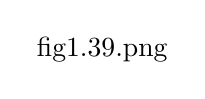
\begin{tikzpicture}
            \node at (0,0) {{fig1.39.png}};
        \end{tikzpicture}
    \end{center}
    \begin{center}
        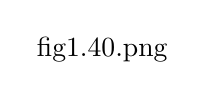
\begin{tikzpicture}
            \node at (0,0) {{fig1.40.png}};
        \end{tikzpicture}
    \end{center}
    \begin{enumerate}
        \item Bar 2 is shifted a small distance $x$ to the left and then released. Find the velocity of the centre of inertia of the system after bar 1 breaks off the wall.
    \end{enumerate}\begin{solution}
    
    \begin{align*}
        \intertext{After releasing, bar 2 acquires velocity \(v_2\), obtained by the energy conservation:}
        \dfrac{1}{2}m_2v_2^2 &= \dfrac{1}{2}\kappa x^2 \quad \text{or} \quad v_2 = x\sqrt{\kappa/m_2} \\
        \intertext{Thus, the sought velocity of C.M.}
        v_C &= \dfrac{0 + m_2 x \sqrt{\kappa/m_2}}{m_1 + m_2} = \dfrac{x \sqrt{m_2 \kappa}}{m_1 + m_2}
    \end{align*}
\end{solution}